\documentclass[../../General.tex]{subfiles}
\begin{document}


\section{Conceptos de solución}
\subsection{Concepto de Solución 1}

El primer concepto de solución agrupa tecnologías económicas ideales para validaciones académicas, pruebas de concepto iniciales o entornos controlados. Estructuralmente, los componentes se protegen dentro de una carcasa fabricada íntegramente en MDF, y su movilidad recae en cuatro ruedas omnidireccionales, aptas para superficies planas, aunque limitadas en campo abierto. Para el despliegue de sus instrumentos climáticos, cuenta con sensores meteorológicos fijos sobre la cubierta y utiliza una plataforma de medición elevable, impulsada por un motor DC y un mecanismo de piñón y cremallera, sobre la cual se aloja un sensor de irradiancia. En el apartado de energía e interfaz, el sistema recibe alimentación a través de conectores Plug Jack y un selector rotativo que dirigen la energía hacia reguladores de voltaje y un Battery Management System acoplado a una batería NiMh. La interfaz física exterior incluye conectores roscados, un panel de luces LED de colores para indicaciones visuales y emite alertas simples a través de un buzzer. Su percepción y navegación se apoyan físicamente en un módulo GPS interno, complementado con el registro de datos en un módulo de memoria FLASH. Finalmente, el control y la lógica se centralizan en un microcontrolador que, a nivel de software, procesa datos mediante tablas de búsqueda, usa control SMC, guía el vehículo mediante el controlador Stanley paralelo y evade obstáculos comparando umbrales temporales.

\begin{figure}[H]
	% Fuerza la alineación izquierda y quita los ":" después del número
	\captionsetup{justification=raggedright, singlelinecheck=false, labelsep=none}
	
	\caption[Diseño general de la solución 1.]{} 
	
	% Vspace negativo opcional para acercar el texto cursivo al número de figura
	\textit{Diseño general de la solución 1.} \par\medskip
	
	\centering
	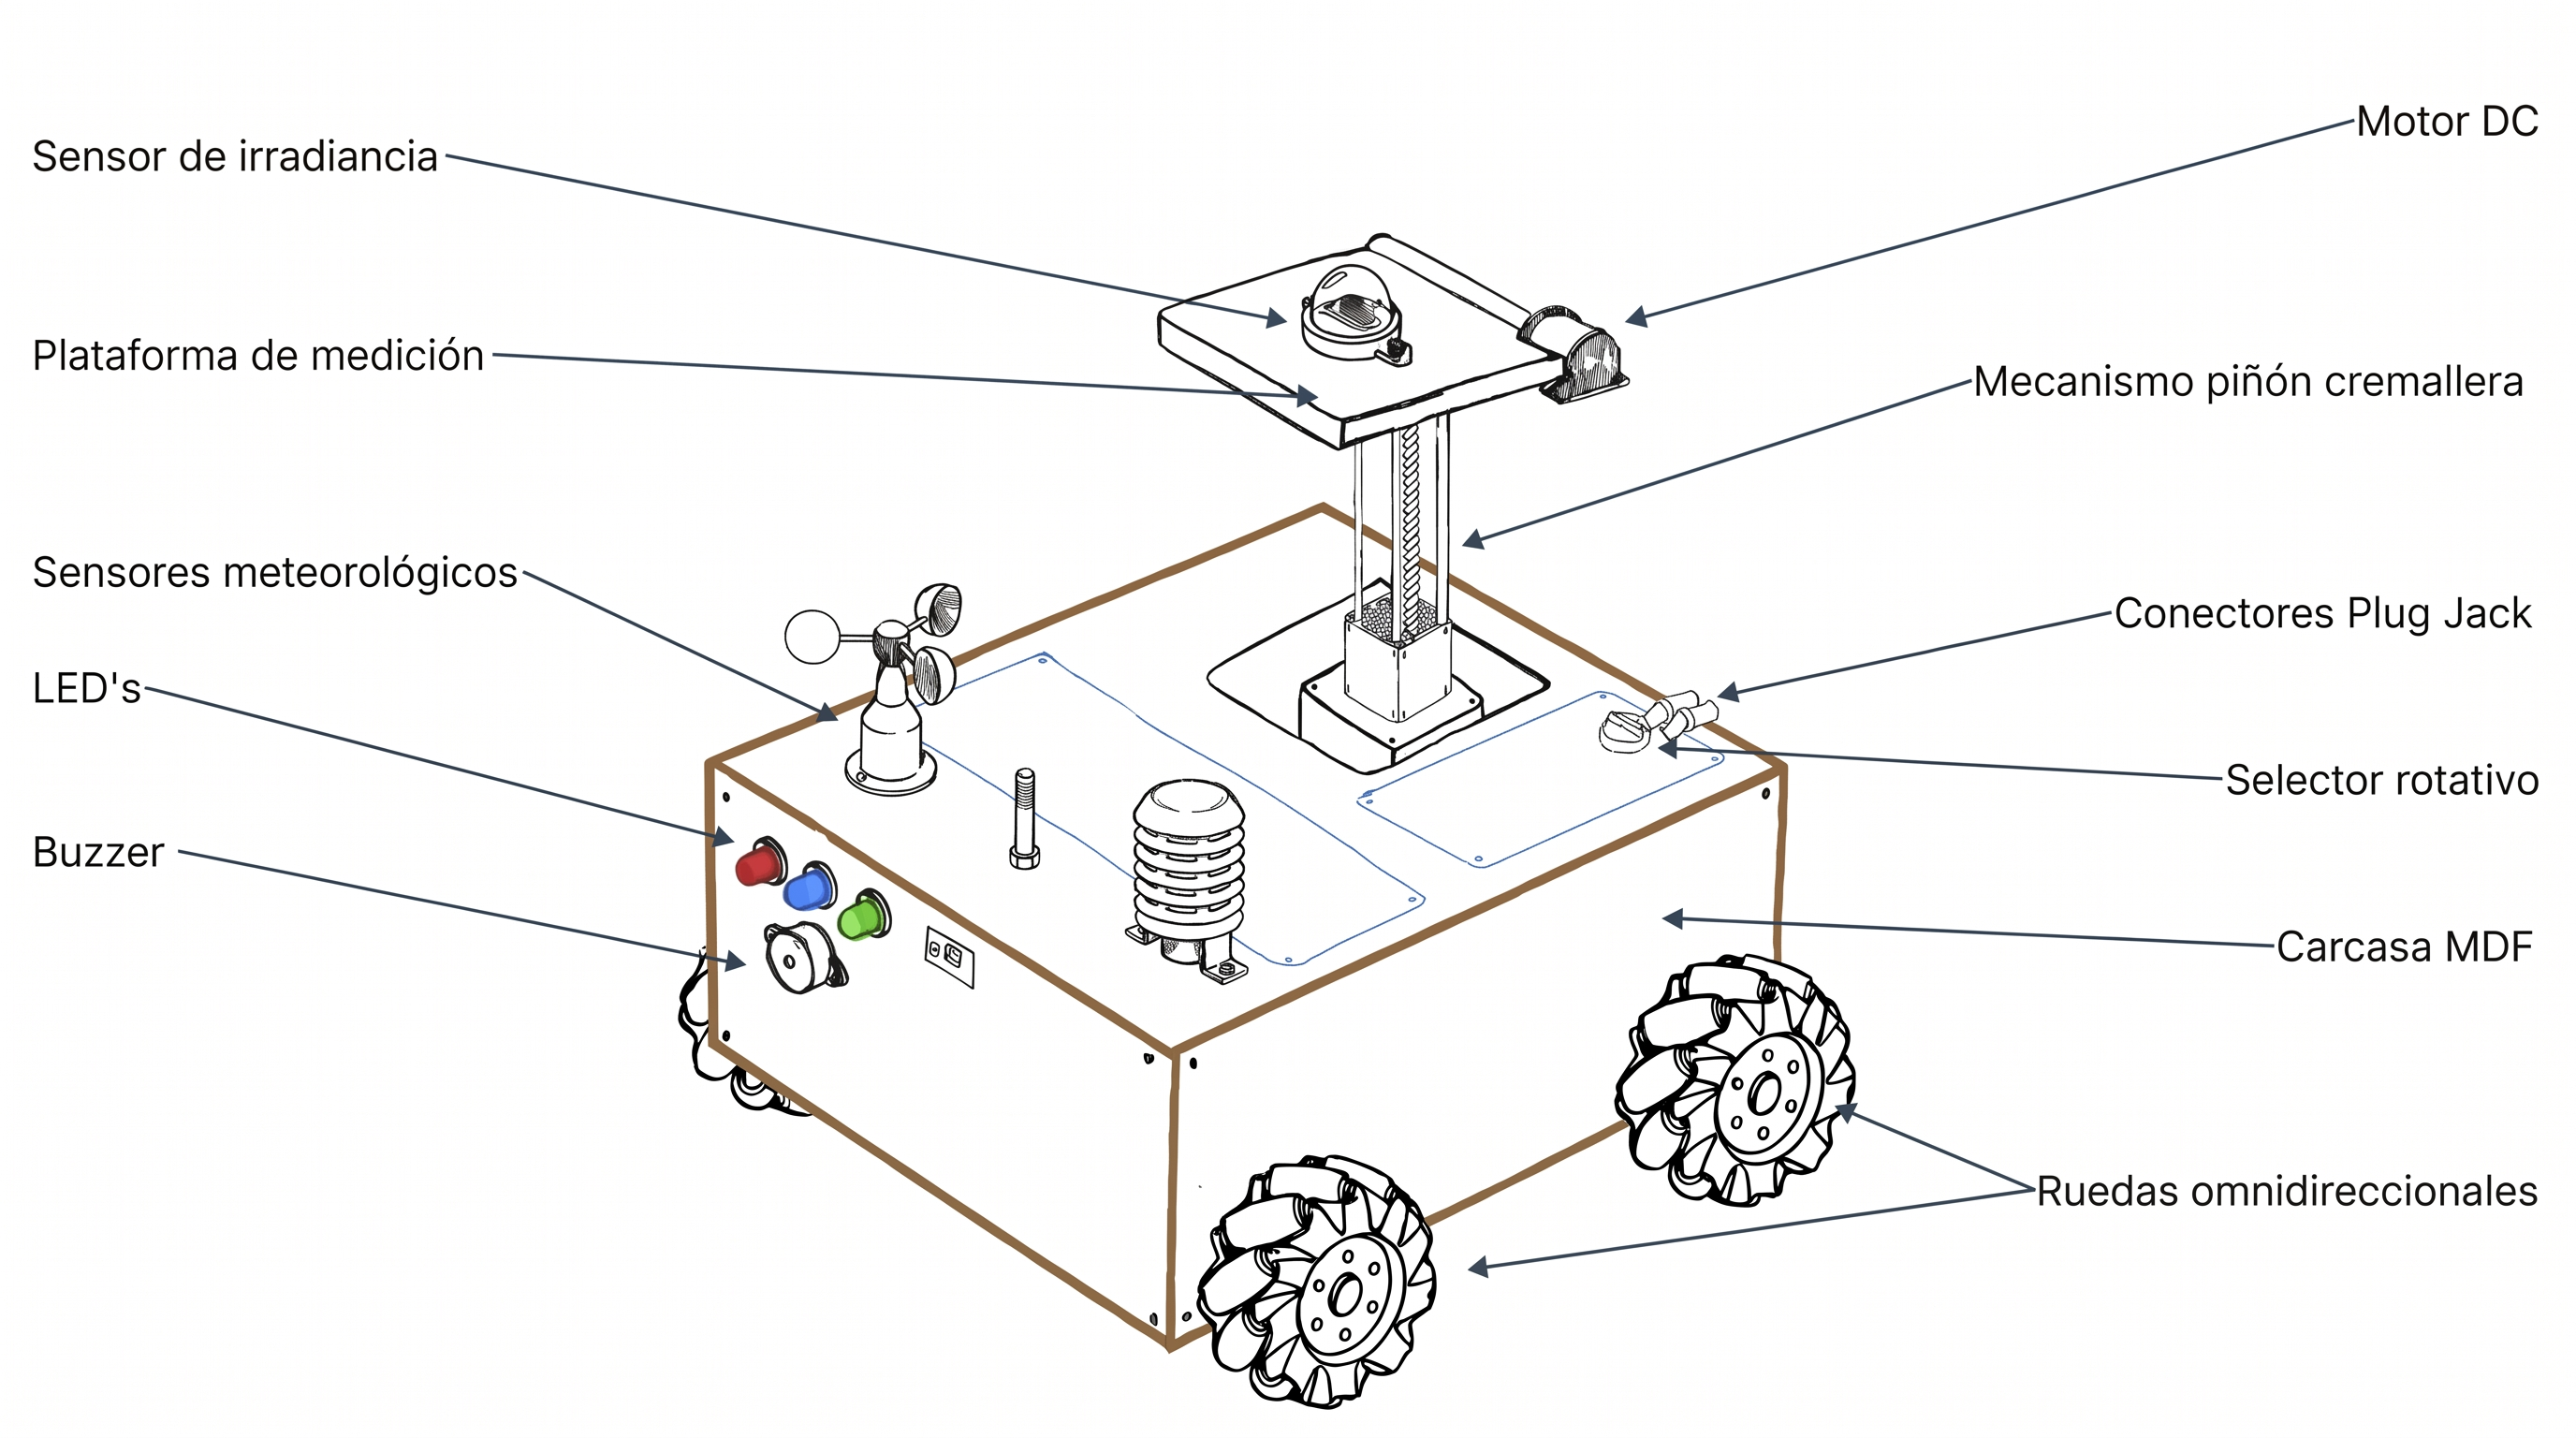
\includegraphics[width=\textwidth]{Recursos/Imagenes/ImagenesConceptos/A-General.jpeg} \par\medskip
	
	\raggedright
	\footnotesize \textit{Nota.} Elaboración propia, asistida con IA generativa.
	\label{fig:AGeneral}
\end{figure}

\begin{figure}[H]
	% Fuerza la alineación izquierda y quita los ":" después del número
	\captionsetup{justification=raggedright, singlelinecheck=false, labelsep=none}
	
	\caption[Diseño interno de la solución 1.]{} 
	
	% Vspace negativo opcional para acercar el texto cursivo al número de figura
	\textit{Diseño interno de la solución 1.} \par\medskip
	
	\centering
	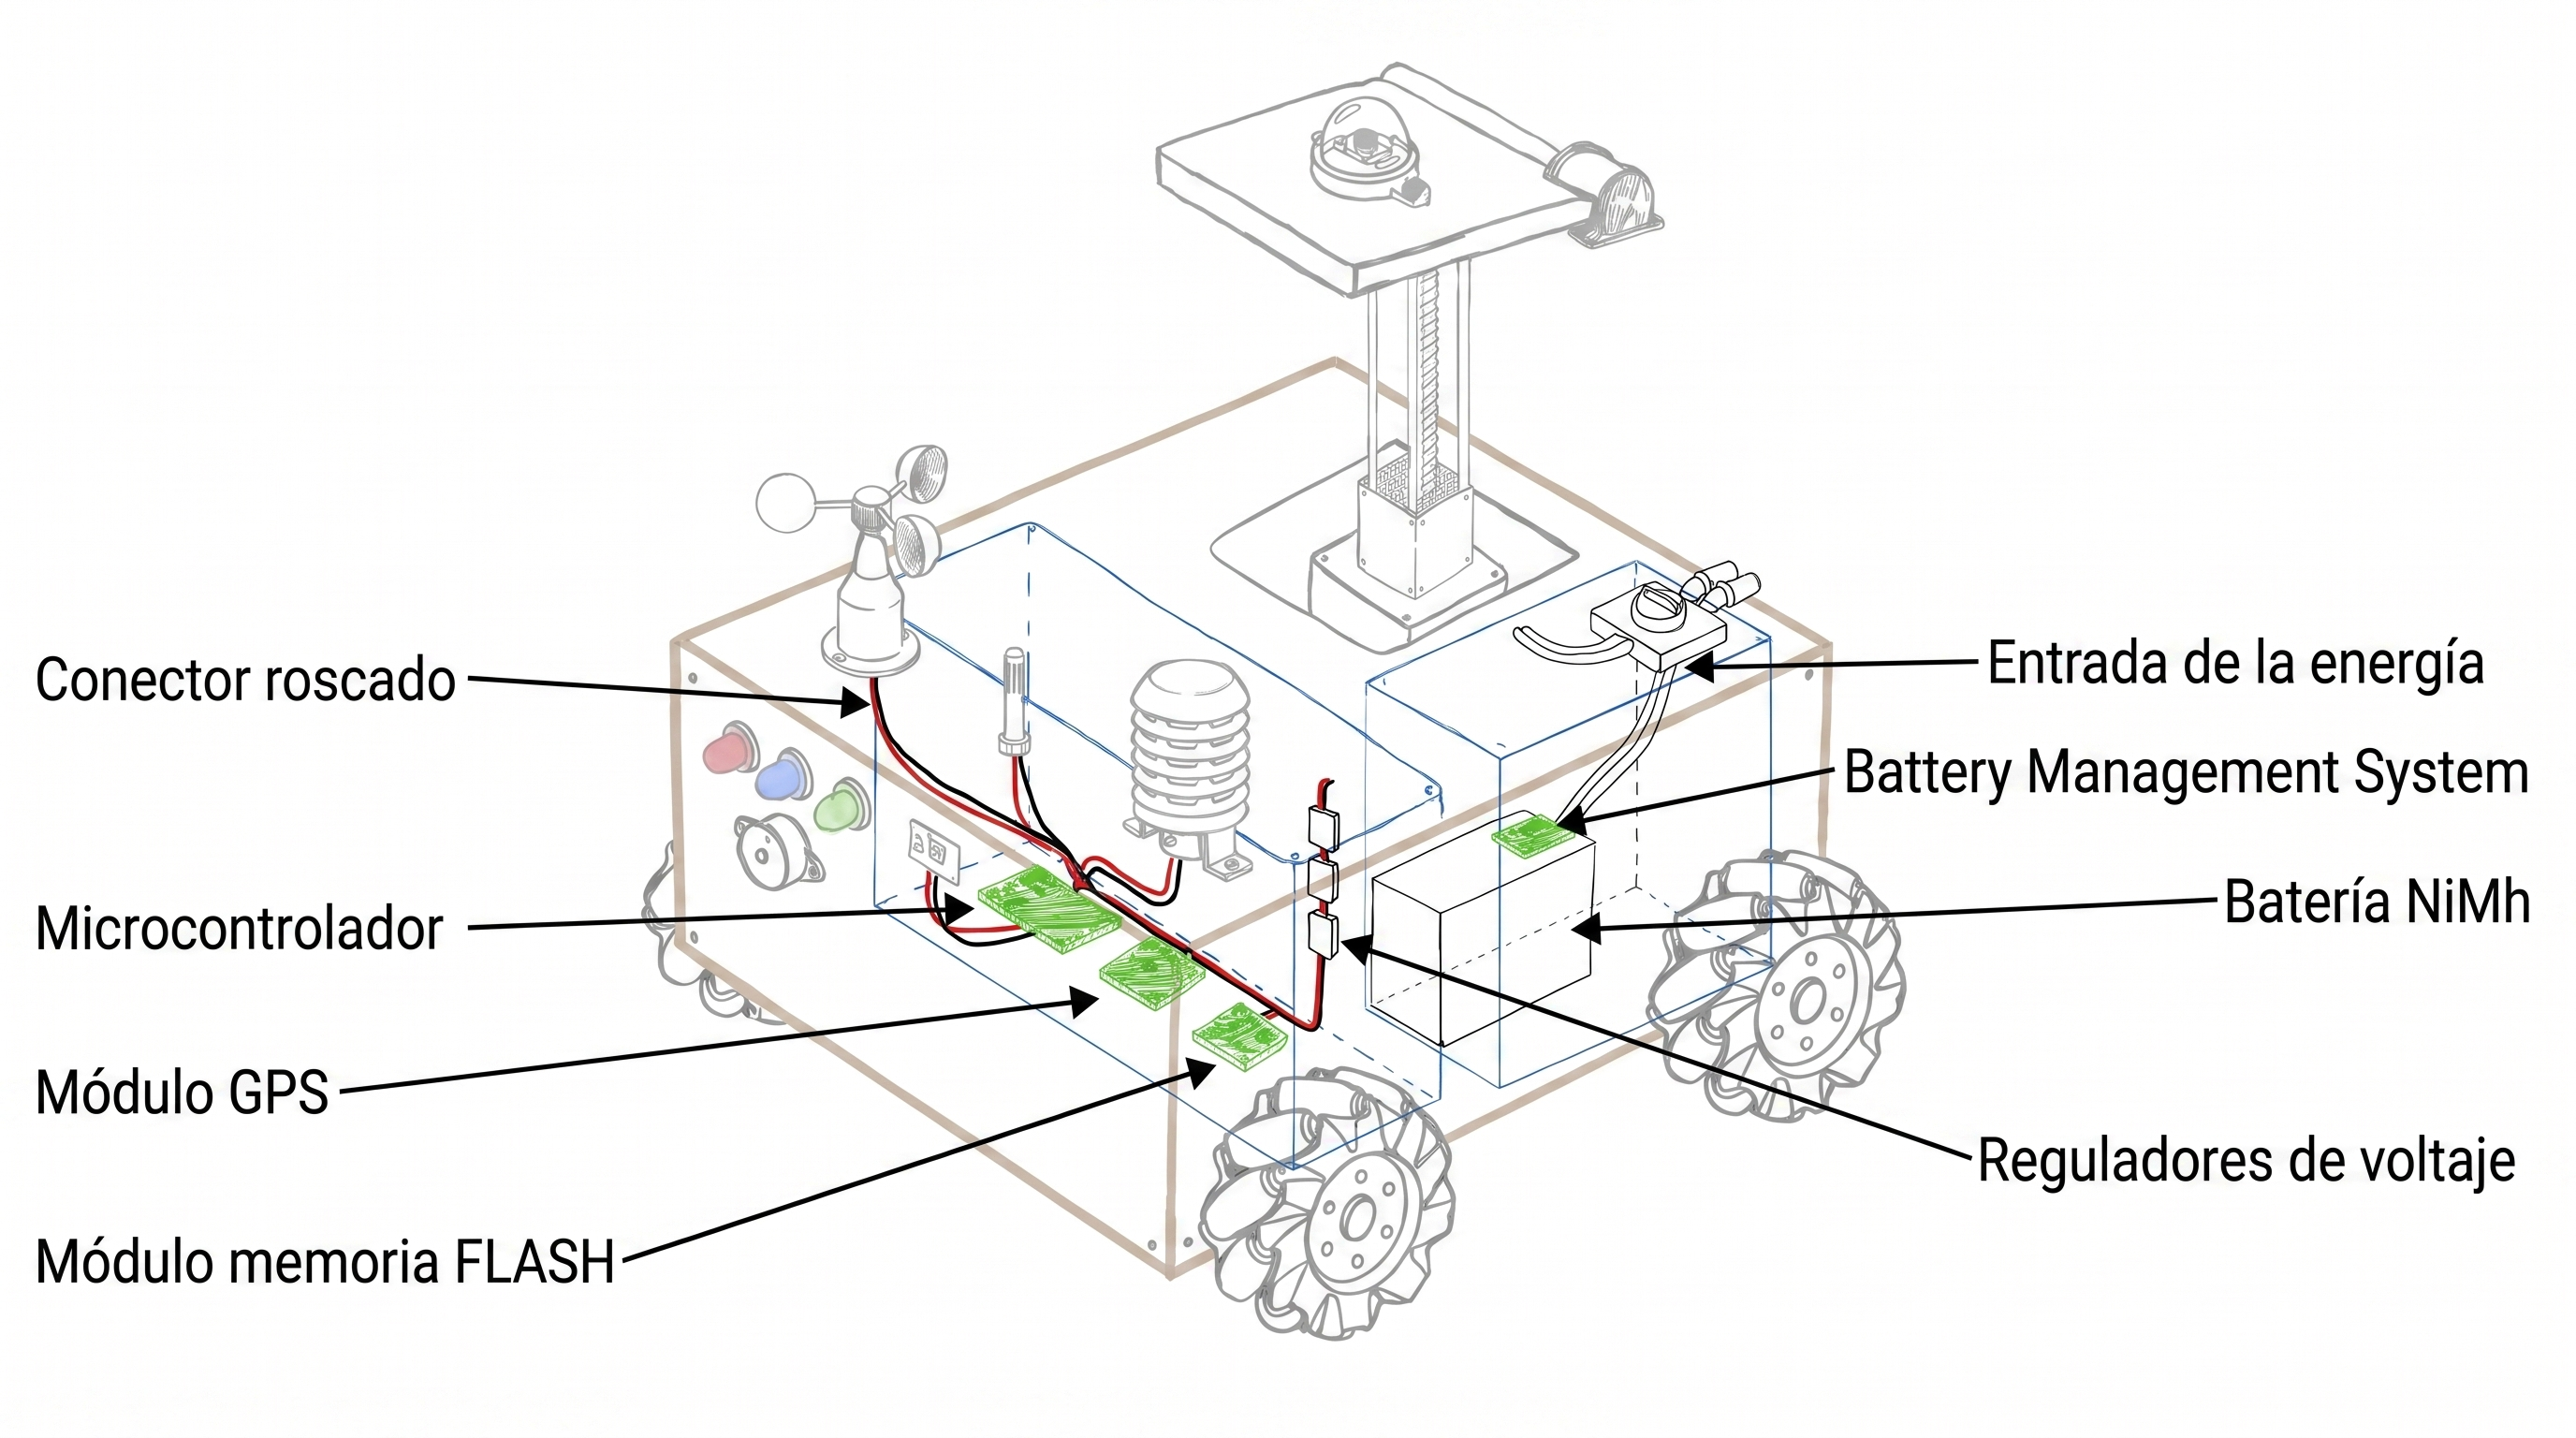
\includegraphics[width=\textwidth]{Recursos/Imagenes/ImagenesConceptos/A-Interno.jpeg} \par\medskip
	
	\raggedright
	\footnotesize \textit{Nota.} Elaboración propia, asistida con IA generativa.
	\label{fig:AInterno}
\end{figure}

\subsection{Concepto de Solución 2}

Este concepto representa un equilibrio óptimo entre robustez técnica, costo y capacidad de procesamiento para entornos de parques solares. A nivel mecánico y estructural, el equipo está construido sólidamente con una carcasa de aluminio y su desplazamiento se da por tracción diferencial mediante cuatro ruedas. Además, cuenta con una plataforma superior de instrumentación móvil, elevada mediante un mecanismo de elevación de tijera, que asegura gran precisión e inamovilidad gracias al mecanismo de tornillo sin-fin y corona accionados por un servomotor DC. En cuanto a energía e interfaz, el robot presenta una alta confiabilidad operando con una batería de iones de litio protegida por sistemas de gestión de batería y reguladores de voltaje internos. Su interfaz exterior emplea borneras industriales para sus conexiones y cuenta con una pantalla LCD junto a una pantalla HMI lateral para interactuar e informar sobre su estado. Para la percepción y exploración, el sistema adquiere datos del entorno mediante sensores meteorológicos y un sensor de irradiancia ubicados en su plataforma elevadiza, emplea un módulo CMOS frontal para la visión por cámara, y transmite o recibe telemetría a través de una antena externa. Finalmente, en cuanto a control y lógica, el cerebro central del robot es una placa SBC que registra la información recopilada en un módulo de memoria microSD.

\begin{figure}[H]
	% Fuerza la alineación izquierda y quita los ":" después del número
	\captionsetup{justification=raggedright, singlelinecheck=false, labelsep=none}
	
	\caption[Diseño general de la solución 2.]{} 
	
	% Vspace negativo opcional para acercar el texto cursivo al número de figura
	\textit{Diseño general de la solución 2.} \par\medskip
	
	\centering
	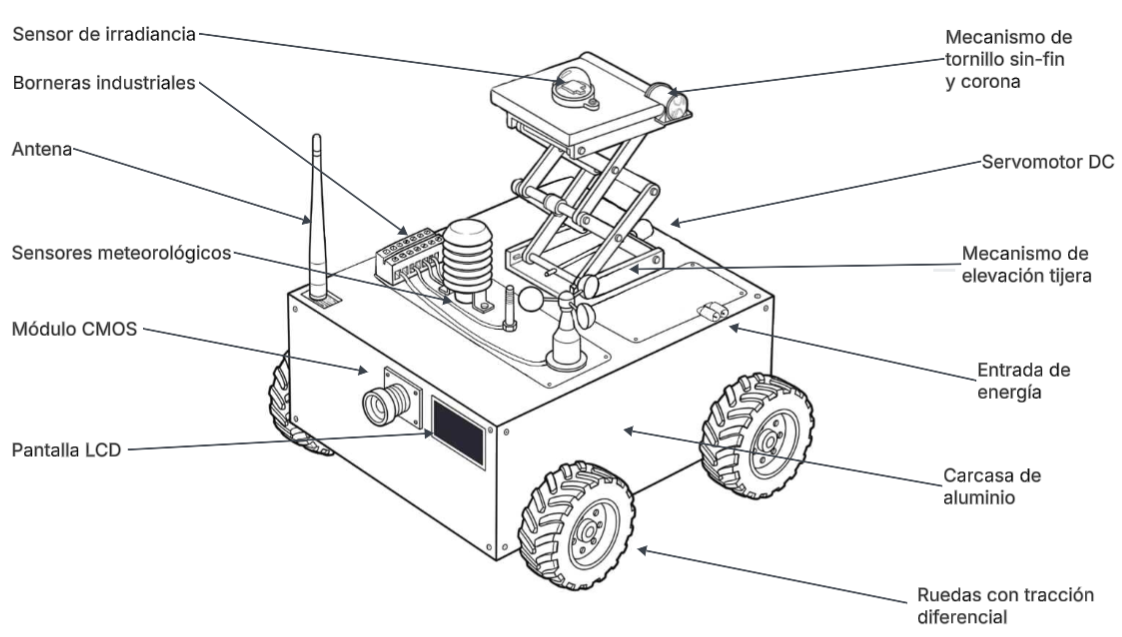
\includegraphics[width=\textwidth]{Recursos/Imagenes/ImagenesConceptos/B-General.png} \par\medskip
	
	\raggedright
	\footnotesize \textit{Nota.} Elaboración propia, asistida con IA generativa.
	\label{fig:BGeneral}
\end{figure}

\begin{figure}[H]
	% Fuerza la alineación izquierda y quita los ":" después del número
	\captionsetup{justification=raggedright, singlelinecheck=false, labelsep=none}
	
	\caption[Diseño interno de la solución 2.]{} 
	
	% Vspace negativo opcional para acercar el texto cursivo al número de figura
	\textit{Diseño interno de la solución 2.} \par\medskip
	
	\centering
	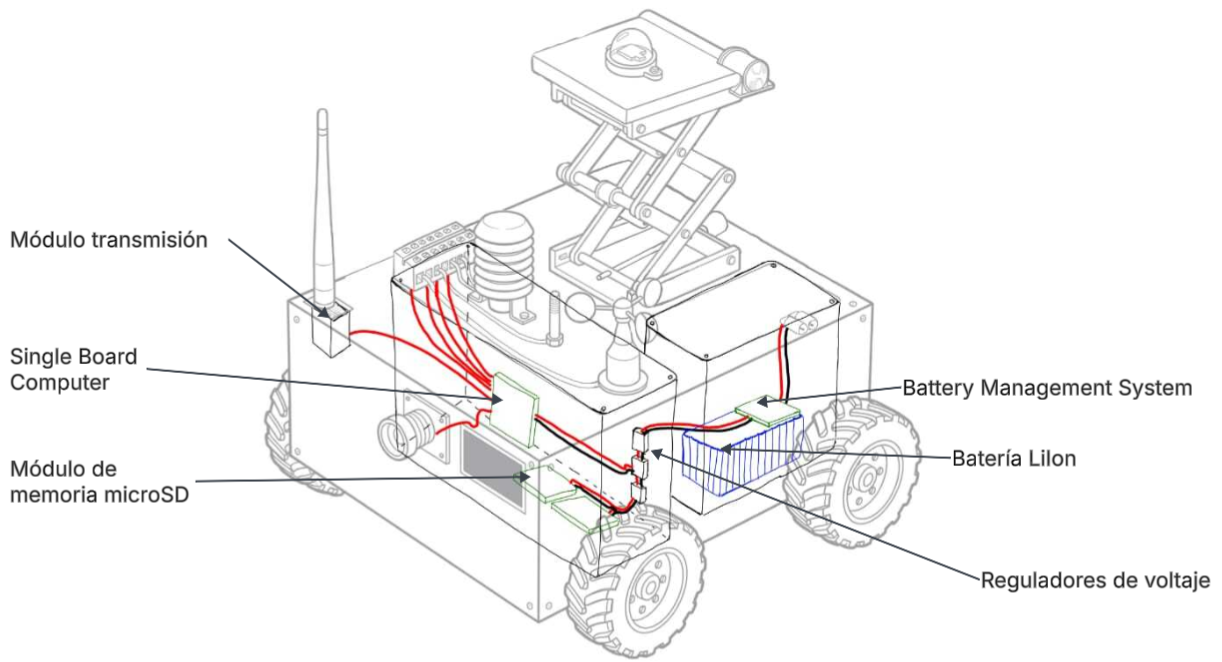
\includegraphics[width=\textwidth]{Recursos/Imagenes/ImagenesConceptos/B-Interno.png} \par\medskip
	
	\raggedright
	\footnotesize \textit{Nota.} Elaboración propia, asistida con IA generativa.
	\label{fig:BInterno}
\end{figure}

\subsection{Concepto de Solución 3}

El tercer concepto de soluciíon corresponde al nivel tecnológico industrial, diseñado para resistir las condiciones topográficas y climáticas más agresivas. Su estructura mecánica emplea un blindaje mediante una carcasa principal de acero y garantiza la movilidad en terrenos accidentados gracias a un sistema de ruedas con tracción de oruga que es impulsado internamente por un motorreductor DC. El equipo integra una plataforma de medición que descansa sobre de una viga elevada mediante un mecanismo de elevación telescópica por un actuador lineal. En el apartado de energía e interfaz, el robot dispone de un sistema de carga exterior mediante contactos magnéticos, reguladores de voltaje internos y se alimenta con una batería LiPo protegida por un Battery Management System. Todo el cableado y la electrónica interna utilizan conexiones herméticas Deutsch, mientras que el chasis exterior se complementa con una pantalla HMI para la interacción directa y una sirena LED de señalización. La percepción y lectura del entorno están a cargo de un sensor LiDAR frontal, apoyado por sensores meteorológicos y un sensor de irradiancia montados en la plataforma superior. Finalmente, el control y la lógica del sistema son gobernados por un PLC, el cual es controlado por un computador industrial (IPC) para procesar eficientemente los datos del entorno, como la segmentación de nubes de puntos del LiDAR, permitiendo así una navegación avanzada.

\begin{figure}[H]
	% Fuerza la alineación izquierda y quita los ":" después del número
	\captionsetup{justification=raggedright, singlelinecheck=false, labelsep=none}
	
	\caption[Diseño general de la solución 3.]{} 
	
	% Vspace negativo opcional para acercar el texto cursivo al número de figura
	\textit{Diseño general de la solución 3.} \par\medskip
	
	\centering
	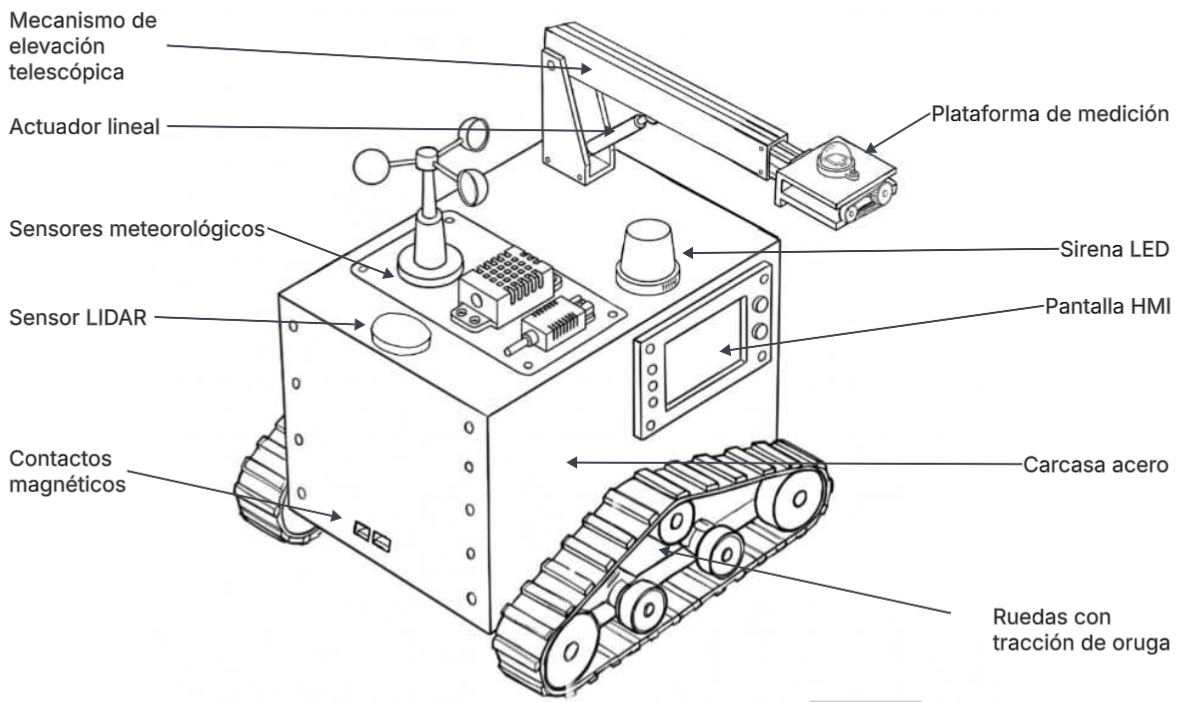
\includegraphics[width=\textwidth]{Recursos/Imagenes/ImagenesConceptos/C-General.png} \par\medskip
	
	\raggedright
	\footnotesize \textit{Nota.} Elaboración propia, asistida con IA generativa.
	\label{fig:CGeneral}
\end{figure}

\begin{figure}[H]
	% Fuerza la alineación izquierda y quita los ":" después del número
	\captionsetup{justification=raggedright, singlelinecheck=false, labelsep=none}
	
	\caption[Diseño interno de la solución 3.]{} 
	
	% Vspace negativo opcional para acercar el texto cursivo al número de figura
	\textit{Diseño interno de la solución 3.} \par\medskip
	
	\centering
	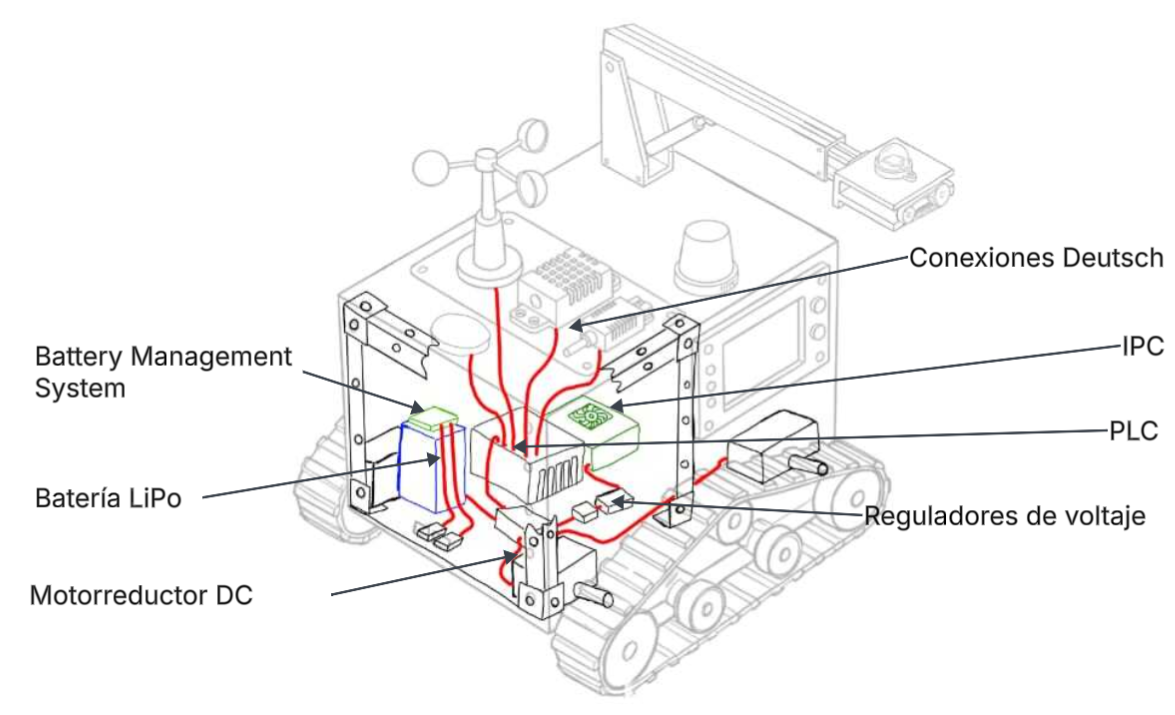
\includegraphics[width=\textwidth]{Recursos/Imagenes/ImagenesConceptos/C-Interno.png} \par\medskip
	
	\raggedright
	\footnotesize \textit{Nota.} Elaboración propia, asistida con IA generativa.
	\label{fig:CInterno}
\end{figure}

\end{document}